% !TEX root = main.tex

\section{モデルに基づく改良型PID制御}

ここではまず,ロボットアームのモデリングについて説明する.
ついで,このモデルに基づいて部分的モデルマッチング法(北森の方法)による
改良型PIDコントローラのパラメータ調整について説明する.

\subsection{ロボットアームのモデリング}
\subsubsection{運動方程式と伝達関数}
ロボットアームの運動方程式は
\begin{equation}
  J \ddot{\theta}(t) = -c \dot{\theta}(t) + \tau(t)
  \tag{4.1}
\end{equation}
で与えられる.ただし,$\tau(t)$ [N·m]: アームの回転軸に加わるトルク,$c$: アームの回転軸の粘性摩擦係数,$J$ [kg·m²]: アームの慣性モーメントである.(4.1)式に,
DC モータ,アンプの特性式やギア比を考慮すると,ロボットアームシステム全体の数学モデルは,
\begin{equation}
  \ddot{\theta}(t) = -a \dot{\theta}(t) + b v(t)
  \tag{4.2}
\end{equation}
という形式となる.ここで,$v(t)$ [V]: モータを駆動させるための指令電圧,
$a, b$: アーム,DC モータ,アンプの特性やギア比に関わるパラメータである.

角度制御を考えた場合,制御量は $\theta(t)$,操作量は $v(t)$ であるから,
$v(s) = \mathcal{L}[v(t)]$ から $\theta(s) = \mathcal{L}[\theta(t)]$ への伝達関数 
$P(s)$ は

\begin{equation}
  P(s) = \frac{\theta(s)}{v(s)} = \frac{b}{s(s+a)}
  \tag{4.3}
\end{equation}

となる.

\subsubsection{パラメータ同定}

(4.3)式に含まれるパラメータ $a$, $b$ は測定器で測ることができない未知パラメータである.
そこで,実験によりパラメータ同定を行う.
\begin{align}
  y_d(t) & = \dot{\theta}(t)
\end{align}とすると(4.2)式は    
\begin{align}                                                                    
  y_d(t) & = -a y_d(t) + b v(t) 
\end{align}となるから,    
\begin{align}                                                                             
  v(s) & = \mathcal{L}[v(t)]
\end{align} から
\begin{align}  
  y_d(s) = \mathcal{L}[y_d(t)]
\end{align}への伝達関数 \(P_d(s)\) は1次遅れ要素
\begin{equation}
  P_d(s) = \left( \frac{y_d(s)}{v(s)} \right) = \frac{b}{s + a} \tag{4.5}
\end{equation}
となる.(4.5)式を1次遅れ要素の標準形で表すと
\begin{equation}
  P_d(s) = \frac{K}{1 + Ts}, \quad T = \frac{1}{a}, \quad K = \frac{b}{a} \tag{4.6}
\end{equation}

であるから,$v(t) = 1$ [V] を加えたときの角速度(単位ステップ応答) $y_d(t) = \dot{\theta}(t)$ は図 4.3 のようになる.
したがって,時定数 $T$,ゲイン $K$ を求めれば,未知パラメータ $a, b$ が次式のように定まる.
\begin{equation}
  a = \frac{1}{T}, \quad b = Ka = \frac{K}{T} \tag{4.7}
\end{equation}

\subsection{部分的モデルマッチング法によるPIDコントローラの設計}
\subsubsection{P-D制御(微分先行型PD制御)}
P-D コントローラ(微分先行型PD コントローラ)
\begin{equation}
  v(t) = k_{\mathrm{P}} e(t) - k_D \frac{d}{dt} \theta(t) \quad \Longleftrightarrow \quad v(s) = k_{\mathrm{P}} e(s) - k_D s \theta(s)
\end{equation}
を用いると,(4.5),(4.8) 式より $\theta^{\text{ref}}(s)$ から $\theta(s)$ への伝達関数は2 次遅れ要素
\begin{equation}
  T(s) = \frac{\omega_n^2}{s^2 + 2 \zeta \omega_n s + \omega_n^2}, \quad \omega_n = \sqrt{b k_{\mathrm{P}}}, \quad \zeta = \frac{a + b k_D}{2 \omega_n}
\end{equation}
となる.したがって,(4.9) 式と2 次遅れ系の標準モデル
\begin{equation}
  y_M(s) = T_M(s) \theta^{\text{ref}}(s), \quad T_M(s) = \frac{\omega_M^2}{s^2 + 2 \zeta_M \omega_M s + \omega_M^2}
\end{equation}
の伝達関数 $T_M(s)$ と完全に一致させるには,比例ゲイン $k_P$,微分ゲイン $k_D$ を
\begin{equation}
  k_P = \frac{\omega_M^2}{b}, \quad k_D = \frac{2 \zeta_M \omega_M - a}{b}
\end{equation}
と定めればよい.

なお,ポテンショメータによって検出された角度には高周波成分の観測雑音(ノイズ)が含まれているため,検出された角度をもとに角速度を算出すると,インパルス状の成分を含んでしまう.そこで,実際には,検出された角度を1次のローパスフィルタ
\begin{equation}
  G_f(s) = \frac{1}{1 + T_f s}
\end{equation}
(4.12)
に通して高周波成分の観測雑音を除去した後,角度信号を微分する必要がある.以上のことを考慮すると,P-Dコントローラは
\begin{equation}
  v(s) = k_{\mathrm{P}} e(s) - k_D G_f(s) s \theta(s) = k_{\mathrm{P}} e(s) - \frac{k_D s}{1 + T_f s} \theta(s)
\end{equation}
(4.13)
となる.

\subsubsection{I-P制御(比例先行型PI制御)}
I-Pコントローラ(比例先行型PIコントローラ)は
\begin{equation}
  v(t) = -k_P \theta(t) + k_I \int_0^t e(\tau) d\tau \quad \Longleftrightarrow \quad v(s) = -k_P \theta(s) + \frac{k_I}{s} e(s) \tag{4.14}
\end{equation}
を用いると,(4.5),(4.14)式より \(\theta(s)\) から \(\theta(s)\) への伝達関数は3次遅れ要素
\begin{equation}
  T(s) = \frac{bk_I}{s^3 + as^2 + bk_{\mathrm{P}} s + bk_I} \tag{4.15}
\end{equation}
となる.ここでは,(4.15)式を2次遅れ系の規範モデル(4.10)式の伝達関数\(T_M(s)\)と近似的に一致させるため,
\begin{equation}
  \frac{1}{T(s)} = 1 + \frac{k_{\mathrm{P}}}{k_I}s + \frac{a}{k_I}s^2 + \frac{1}{bk_I}s^3 \tag{4.16}
\end{equation}
\begin{equation}
  \frac{1}{T_M(s)} = 1 + \frac{2\zeta_M}{\omega_M}s + \frac{\omega_M^2}{\omega_M^2}s^2 \tag{4.17}
\end{equation}
の2次までの項が一致するように比例ゲイン\(k_P\),積分ゲイン\(k_I\)を次式のように決定する.
\begin{equation}
  k_P = \frac{2\zeta_M \omega_M a}{b}, \quad k_I = \frac{\omega_M^2 a}{b} \tag{4.18}
\end{equation}
このように規範モデルと部分的に一致させるようなパラメータ調整法を部分的モデルマッチング法と呼ぶ.

\subsubsection{I-PD 制御(比例・微分先行型 PID 制御)}

I-PD コントローラ(比例・微分先行型 PID コントローラ)
\begin{equation}
  v(t) = -k_P \theta(t) + k_I \int_0^t e(\tau) d\tau - k_D \frac{d\theta(t)}{dt} \quad \Longleftrightarrow \quad v(s) = -k_P \theta(s) + \frac{k_I}{s} e(s) - k_D s \theta(s) \tag{4.19}
\end{equation}
を用いると,(4.5),(4.19)式より \(\theta(s)\) から \(\theta(s)\) への伝達関数は3次遅れ要素
\begin{equation}
  T(s) = \frac{b k_I}{s^3 + (a + b k_D)s^2 + b k_P s + b k_I} \tag{4.20}
\end{equation}
となる.したがって,(4.20)式を規範モデル
\begin{equation}
  y_M(s) = T_M(s) \theta_{\mathrm{ref}}(s), \quad T_M(s) = \frac{\omega_M^3}{s^3 + \alpha_{M2} \omega_M s^2 + \alpha_{M1} \omega_M^2 s + \omega_M^3} \tag{4.21}
\end{equation}
の伝達関数 \(T_M(s)\) と完全に一致させるには
\begin{equation}
  k_P = \frac{\alpha_{M1} \omega_M^2}{b}, \quad k_I = \frac{\omega_M^3}{b}, \quad k_D = \frac{\alpha_{M2} \omega_M - a}{b} \tag{4.22}
\end{equation}
と選べばよい.ただし,\(\omega_M\) は速度応答性に関するパラメータ,\(\alpha_{M1}\),\(\alpha_{M2}\) は減衰性に関するパラメータであり,
\begin{equation}
  \begin{array}{ll}
    \text{バターワース標準形}: & \alpha_{M1} = 2, \quad \alpha_{M2} = 2       \\
    \text{二項係数標準形}:     & \alpha_{M1} = 3, \quad \alpha_{M2} = 3       \\
    \text{ITAE 最小標準形}:    & \alpha_{M1} = 2.15, \quad \alpha_{M2} = 1.75 \\
  \end{array}
\end{equation}
が用いられることが多い.なお,ITAE は Integral of Time multiply Absolute Error の略字である.
実際には高周波成分の観測雑音を除去するため,次式のI-PDコントローラを用いることになる.
\begin{equation}
  v(s) = -k_P \theta(s) + \frac{k_I}{s}e(s) - \frac{k_D s}{1 + T_f s} \theta(s) \tag{4.23}
\end{equation}


\newpage

\section{実験2: 改良型PID制御の比較}
\subsection{ローパスフィルタによる観測雑音除去とパラメータ同定}

(1) 図5.1のSimulinkモデル“ex.ident.slx”を作成し,ディレクトリ \texttt{D:\#student\_5S\#group01\#ident} に保存する.図5.1におけるブロックTransfer Fcnはローパスフィルタ \( G_f(s) = \frac{1}{1 + 0.01s} \) を表している.

ビルドを行い,エラーがないことを確認した後,printコマンドにて“ex.ident.pdf”という名前のpdfファイルを生成し,デスクトップ上の “bcpdfcrop-multi.bat” により余白を取り除く.

(2) Scopeをダブルクリックして開き,リアルタイムで角度データを観測できるようにする.レンジは付録A.2の図A.5に合わせる.

(3) オシロスコープをUniversal Power Moduleの“S1”と“GND”に接続し,センサ電圧が0[V]となる位置にアームを動かす.

(4) “ex.ident.slx”を実行する.実行終了後,
\begin{verbatim}
>> save ident_data t y dy dyf
\end{verbatim}
と入力し,matファイル“ident\_data.mat”にデータを保存する.

(5) 配布するMファイル
\begin{verbatim}
ident_para.m
\end{verbatim}
を実行することによって,実験結果のグラフを描くとともに定常値 \( y_{\infty} = K \) および \( y_{\infty} = K \) の63.2\%に至るまでの時間 \( T \) を抽出する.この結果を基に未知パラメータ \( a \) , \( b \) を定め,表5.1に記入せよ.


\subsubsection{実験結果}
以下に結果を示す.

\begin{table}[h]
  \centering
  \caption{同定されたパラメータの値}
  \begin{tabular}{|c|c|c|c|}
    \hline
    ゲイン \( K \) & 時定数 \( T \) & \( a \) & \( b \) \\ \hline
    1.46           & 0.046          & 21.7    & 31.8    \\ \hline
  \end{tabular}
\end{table}

\begin{figure}[h]
  \centering
  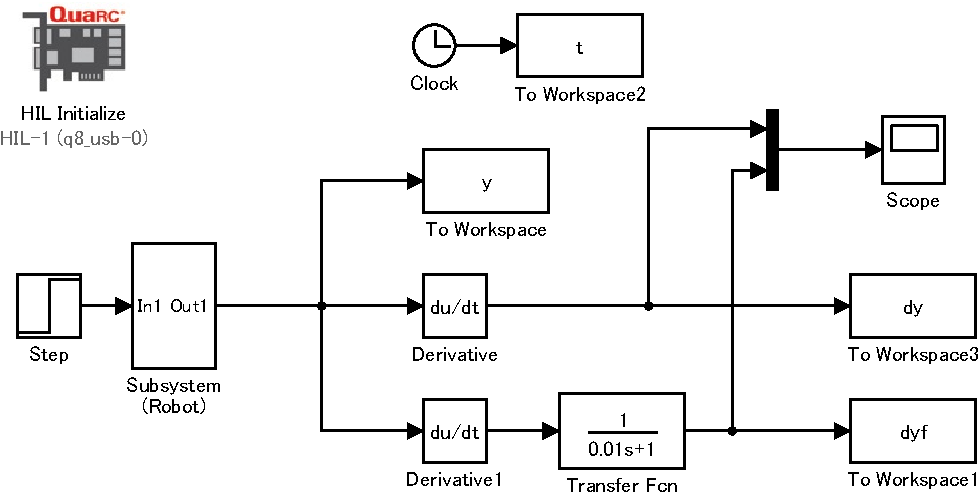
\includegraphics[scale=0.7]{sozai/ex_ident-crop.pdf}
  \caption{ex\_ident}
\end{figure}

\begin{figure}[h]
  \centering
  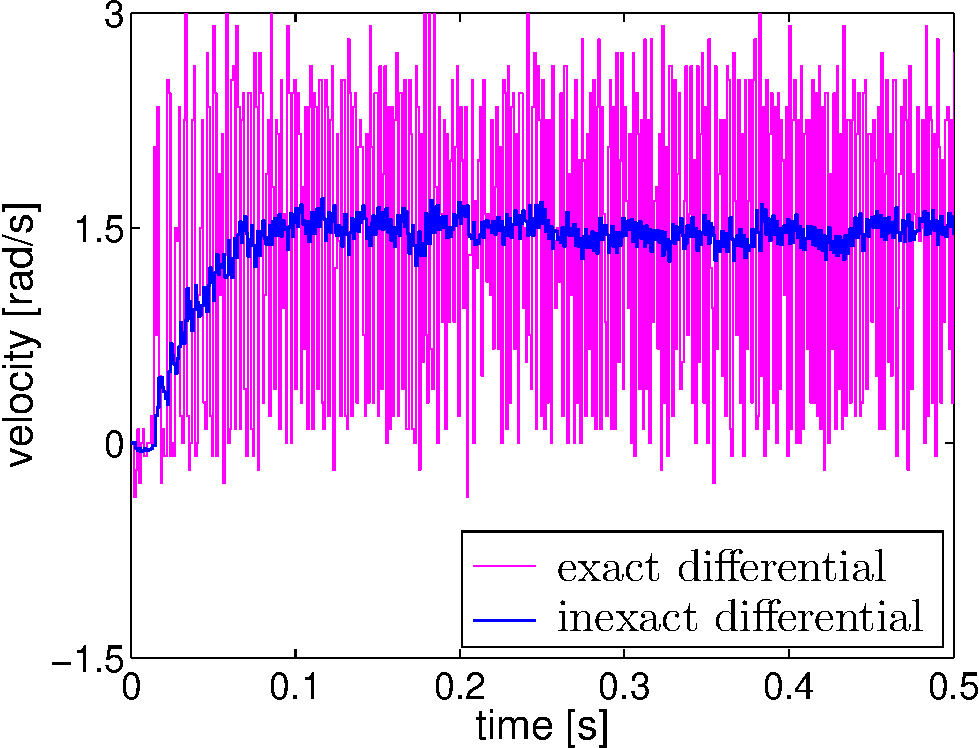
\includegraphics[scale=0.5]{sozai/figure_lowpass-crop.pdf}
  \caption{figure\_lowpass}
\end{figure}

\begin{figure}[h]
  \centering
  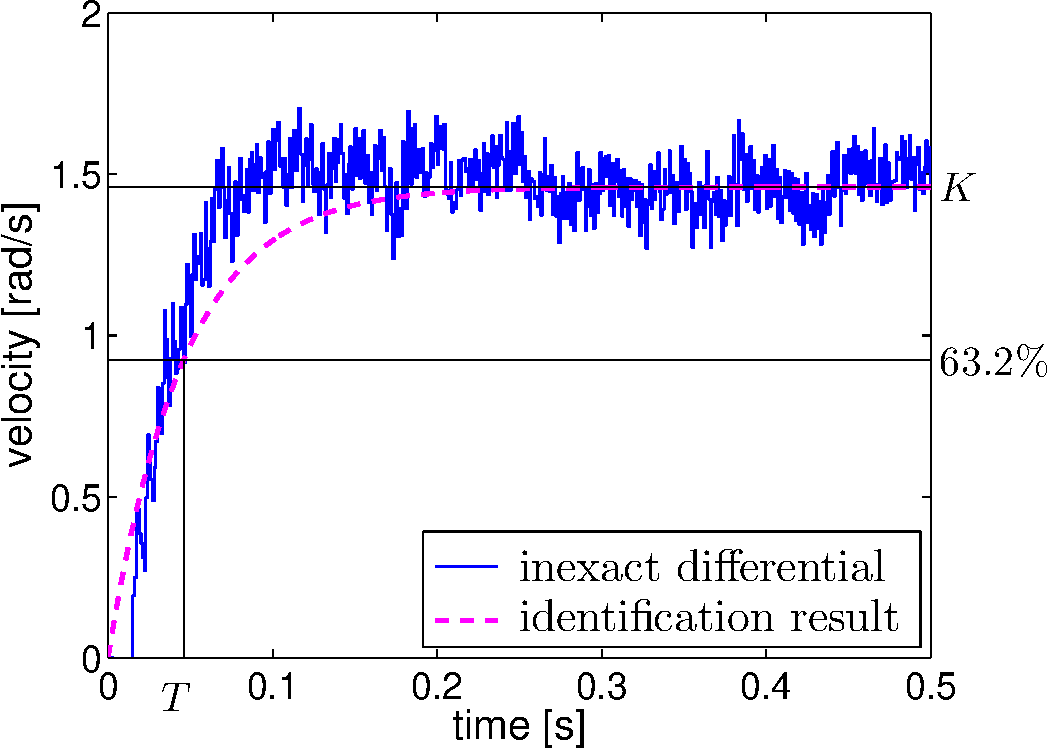
\includegraphics[scale=0.5]{sozai/figure_ident-crop.pdf}
  \caption{figure\_ident}
\end{figure}

\newpage

\subsubsection{実験考察}

実験により得られたパラメータは,表に示すように,ゲイン \( K = 1.46 \),
時定数 \( T = 0.046 \) ,および未知パラメータ \( a = 21.7 \),\( b = 31.8 \) である.
図5.2の結果より,ローパスフィルタを適用していない場合(exact differential)は,
観測雑音により信号に大きな振動が生じているのが確認できる.
一方,ローパスフィルタを適用した場合(inexact differential)では,
結果図5.3から得られたゲイン \( K = 1.46 \) は,
システムが入力ステップ応答に対して約63.2\%に達する値であり,
実験により同定された時定数 \( T = 0.046 \) は,
システムがこの値に収束するまでの応答時間を表している.
また, \( \frac{1}{\omega} = \frac{1}{100} \approx 0.01 \, 
\text{s} \) であるのに対し,同定されたシステムの時定数は \( T = 0.046 \, \text{s} \)
であることがわかる.

そして,カットオフ周波数は
\[
  f = \frac{\omega}{2 \pi} \approx 15.9 \, \text{[rad/s]}
\]
となる.
したがって,フィルタのカットオフ周波数はノイズ周波数 \( 100 \, \text{[rad/s]} \) よりも
低く設定されており,このフィルタによってノイズが効果的に減衰されると考えられる.
図5.2に示されるように,exact differential(フィルタ未適用)の場合には
高周波成分による大きな振動が観察されたが,
inexact differential(フィルタ適用)の場合にはノイズが減衰され,
信号が滑らかになっている.


\subsection{P-D 制御}

\begin{enumerate}
  \item (4.11) 式にしたがって P-D コントローラ (4.13) 式のパラメータを定め,表 5.2 を完成させよ.
        
  \item 図 5.2 の Simulink モデル "ex.pdcont.slx" を作成し,ディレクトリ D:\#student.5S\#group01\#pdcont に保存する.ただし,"Subsystem (P-D Controller)" の内部は各自作成する(角速度 $\dot{\theta}$ はローパスフィルタ $G_f(s) = \frac{1}{1 + 0.01s}$ に通す).
        
  \item 次に,表 5.2 に示す比例ゲイン $k_{\mathrm{P}}$,微分ゲイン $k_{\mathrm{D}}$ を,コマンドウィンドウで
        
        \(>> k_{\mathrm{P}} = ***; k_{\mathrm{D}} = ***;\)
        
        と入力(*** には表 5.2 の数字を入力する)した後,ビルドを行い,エラーがないことを確認する.
        また,"ex.pdcont.pdf" という名前の pdf ファイルを生成し,デスクトップ上の 
        "bcpdfcrop-multi.bat" により余白を取り除く.
        
  \item Scope と Scope1 を開き,リアルタイムで角度と操作量を観測できるようにする.レンズは付録 A.2 の図 A.6 に合わせる.
        
  \item センサ電圧が 0 [V] となる位置にアームを動かし,"ex.pdcont.slx" を実行する.実行ss終了後,コマンドウィンドウで
        
        
        >> save pdcont\_data1 t u y \(k_{\mathrm{P}} k_{\mathrm{D}}\)
        
        
        と入力し,データを
        
        \begin{itemize}
          \item "pdcont.data1.mat" ($\omega_M = 15, \zeta_M = 0.3$)
          \item "pdcont.data2.mat" ($\omega_M = 15, \zeta_M = 0.7$)
          \item "pdcont.data3.mat" ($\omega_M = 15, \zeta_M = 1$)
        \end{itemize}
        
        という名前の mat ファイルでディレクトリ D:\#student.5S\#group01\#pdcont に保存する.最後に,配布する M ファイル
        
        "autoplot\_pdcont.m"
        
        を実行することによって,MATLAB 上でグラフを作成する.グラフの pdf ファイルは自動的に生成される.
        
  \item 目標値を 0 に設定(Step の最終値を "0" に設定)し,また,終了時間を "inf" に設定する.$\omega_M$, $\zeta_M$ を表 5.2 のように与えた後,アームを平らに 45 [deg] 程度動かしてから手を放すとき,アームがどのように応答するか調べよ.
\end{enumerate}


\subsubsection{実験結果}
以下に結果を示す.

\begin{figure}[h]
  \centering
  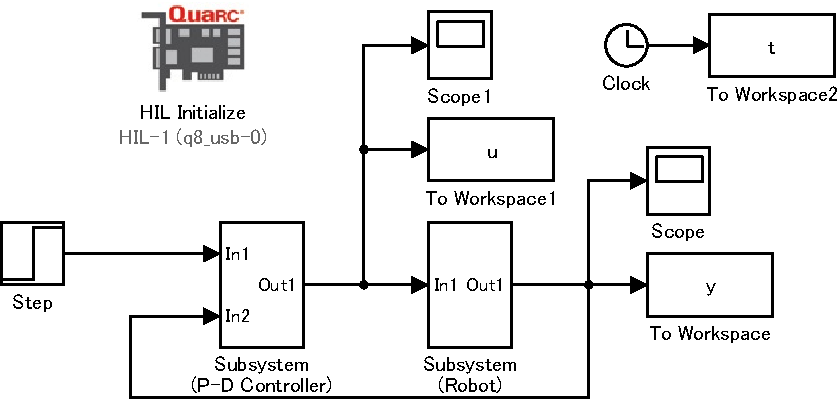
\includegraphics[scale=1]{sozai/ex_pdcont-crop.pdf}
  \caption{ex\_pdcont}
\end{figure}

\begin{table}[h]
  \centering
  \caption{P-D コントローラ}
  \begin{tabular}{|c|c|c|c|}
    \hline
    固有角周波数 $\omega_M$ & 減衰係数 $\zeta_M$ & 比例ゲイン $k_{\mathrm{P}}$ & 微分ゲイン $k_{\mathrm{D}}$ \\
    \hline
    15                      & 0.3                & 7.075                       & -0.399                      \\
    15                      & 0.7                & 7.075                       & -0.022                      \\
    15                      & 1                  & 7.075                       & 0.261                       \\
    \hline
  \end{tabular}
\end{table}

\begin{figure}[h]
  \centering
  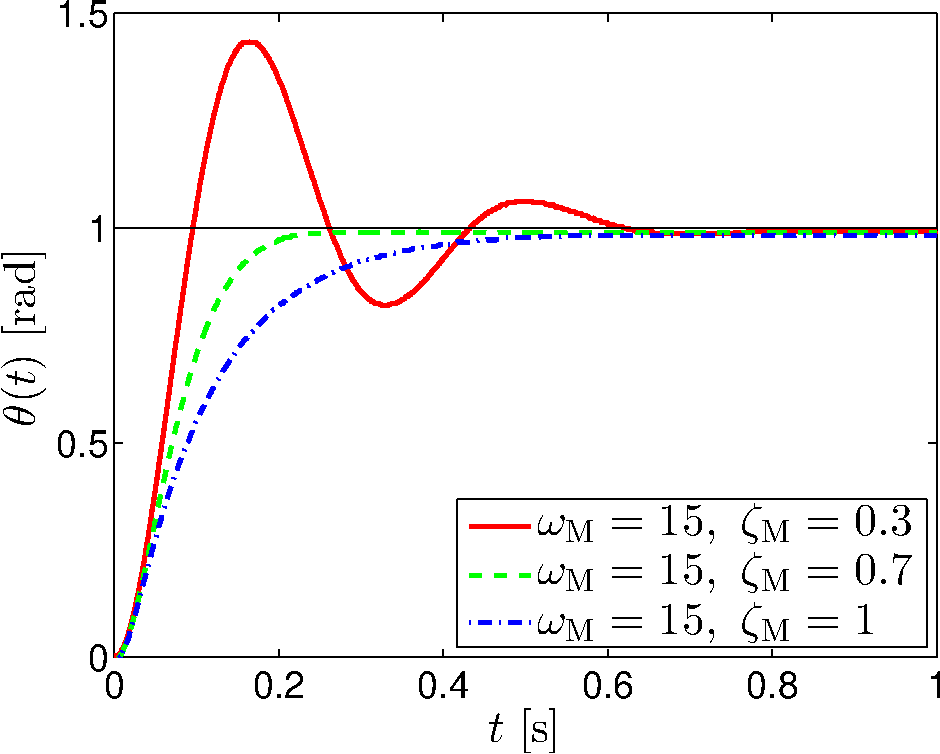
\includegraphics[scale=0.5]{sozai/figure_pdcont_angle-crop.pdf}
  \caption{ex\_pdcont}
\end{figure}

\begin{figure}[h]
  \centering
  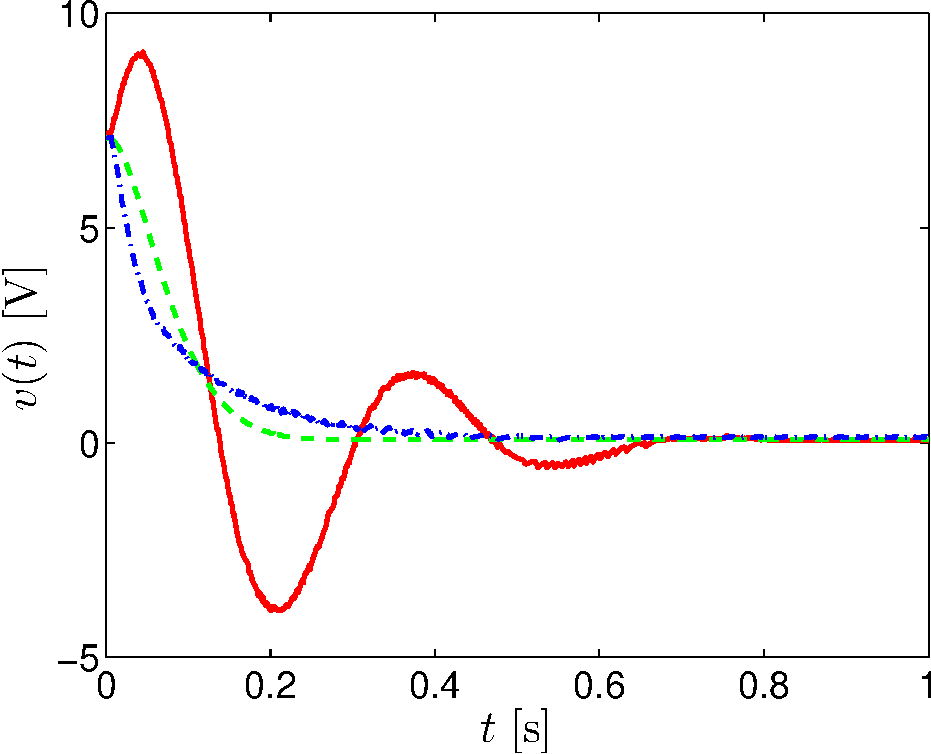
\includegraphics[scale=0.5]{sozai/figure_pdcont_volt-crop.pdf}
  \caption{ex\_pdcont}
\end{figure}

\newpage

(5) 減衰係数が大きくなるに連れ,即応性がなくなり,ゆっくりになりダンパの動きが見られた.

\subsubsection{実験考察}
微分動作は,制御対象の誤差の時間変化を考慮し,制御入力を調整するものである.
これにより応答の速度が向上し,オーバーシュートの抑制や立ち上がり時間の短縮が期待できる.
微分動作を加えることで,過渡応答が改善され,立ち上がり時の急激な変動が抑制されると考えられる.

次に,規範モデル式 (4.10) に基づくステップ応答と実験結果における定常偏差の違いについて述べる.
理論的な規範モデルは,理想的な条件での応答を示しているが,PD制御である場合,定常偏差が残る可能性がある.
このことは次の最終値の定理からも確認できる.
\[
  \lim_{t \to \infty} e(t) = \lim_{s \to 0} s E(s)
\]
積分動作がない場合,\( e(t) \) はゼロに収束せず,
定常偏差が残存することになる.
次に,減衰係数を変化させたときのアームの挙動について,
マスバネダンパ系の視点から考察する.マスバネダンパ系の運動方程式は以下のように表される.
\[
  m \ddot{z} + c \dot{z} + k z = f
\]
これを \( f \) について解くと,
\[
  f = m \ddot{z} + c \dot{z} + k z
\]
となる.ここで,\( m \) は質量,\( c \) はダンパ係数(減衰係数に関係),\( k \) はバネ定数
(固有角周波数に関係)である.
この系の伝達関数 \( P(s) \) は,出力を \( z(s) \) ,入力を \( f(s) \) として
\[
  P(s) = \frac{z(s)}{f(s)} = \frac{1}{m s^2 + c s + k}
\]
と表される.
さらに,この系を2次遅れ系の標準形に変換するため,分母の式を整理すると
\[
  P(s) = \frac{\frac{1}{m}}{s^2 + \frac{c}{m} s + \frac{k}{m}}
\]
となる.ここで,2次遅れ系の標準形
\[
  P(s) = \frac{\omega_n^2}{s^2 + 2 \zeta \omega_n s + \omega_n^2}
\]
と比較すると,固有角周波数 \( \omega_n \) と減衰係数 \( \zeta \) はそれぞれ以下のように表されることが
わかる.
\[
  \omega_n = \sqrt{\frac{k}{m}}, \quad \zeta = \frac{c}{2 \sqrt{m k}}
\]
これにより,バネ定数 \( k \) を変化させると固有角周波数 \( \omega_n \) が変化し,
ダンパ係数 \( c \) を変化させると減衰係数 \( \zeta \) が変化することがわかる.


\subsection{I-P制御}
\begin{enumerate}
  \item (4.18)式にしたがってI-Pコントローラ(4.14)式のパラメータを定め,表5.3を完成する.
  \item 図5.3のSimulinkモデル“ex\_ipcont.slx”を作成し,ディレクトリD:\#student\_5S\#group01\#ipcontに保存する.ただし,“Subsystem (I-P Controller)”の内容は各自で考える.
  \item 表5.3の比例ゲイン$k_{\mathrm{P}}$,積分ゲイン$k_{\mathrm{I}}$をコマンドウィンドウで
        \begin{verbatim}
  >> kP = ***; kI = ***;
  \end{verbatim}
        と入力し(***には表5.3の数値を入力する),ビルドを行い,エラーがないことを確認する.また,“ex\_ipcont.pdf”という名前のpdfファイルを生成し,デスクトップ上の“bcpdfcrop-multi.bat”により余白を取り除く.
        
  \item ScopeとScope1を開き,リアルタイムで角度と操作量を観測できるようにする.レンズは付録A.2の図A.7に合わせる.
        
  \item センサ電圧が0[V]となる位置にアームを動かし,“ex\_ipcont.slx”を実行する.実行終了後,コマンドウィンドウで
        \begin{verbatim}
  >> save ipcont_data1 t u y kP kI
  \end{verbatim}
        と入力し,データを
        \begin{itemize}
          \item “ipcont\_data1.mat” ($\omega_M = 15, \zeta_M = 0.3$)
          \item “ipcont\_data2.mat” ($\omega_M = 15, \zeta_M = 0.7$)
          \item “ipcont\_data3.mat” ($\omega_M = 15, \zeta_M = 1$)
        \end{itemize}
        という名前のmatファイルでディレクトリD:\#student\_5S\#group01\#ipcontに保存する.最後に,配布するMファイル
        \begin{verbatim}
  autoplot-ipcont.m
  \end{verbatim}
        を実行することによって,MATLAB上でグラフを作成する.グラフのpdfファイルは自動的に生成される.
        
\end{enumerate}

\subsubsection{実験結果}
\begin{figure}[h]
  \centering
  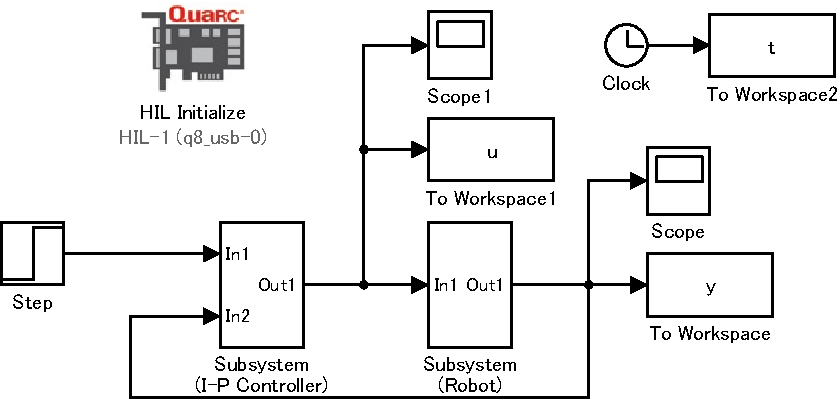
\includegraphics[scale=1]{sozai/ex_ipcont-crop.pdf}
  \caption{ex\_ipcont}
\end{figure}

\begin{table}[h]
  \centering
  \caption{I-Pコントローラ}
  \begin{tabular}{|c|c|c|c|}
    \hline
    固有角周波数$\omega_M$ & 減衰係数$\zeta_M$ & 比例ゲイン$k_{\mathrm{P}}$ & 積分ゲイン$k_{\mathrm{I}}$ \\
    \hline
    15                     & 0.3               & 6.14150                    & 153.53773                  \\
    15                     & 0.7               & 14.33018                   & 153.53773                  \\
    15                     & 1                 & 20.47169                   & 153.53773                  \\
    \hline
  \end{tabular}
\end{table}

\begin{figure}[h]
  \centering
  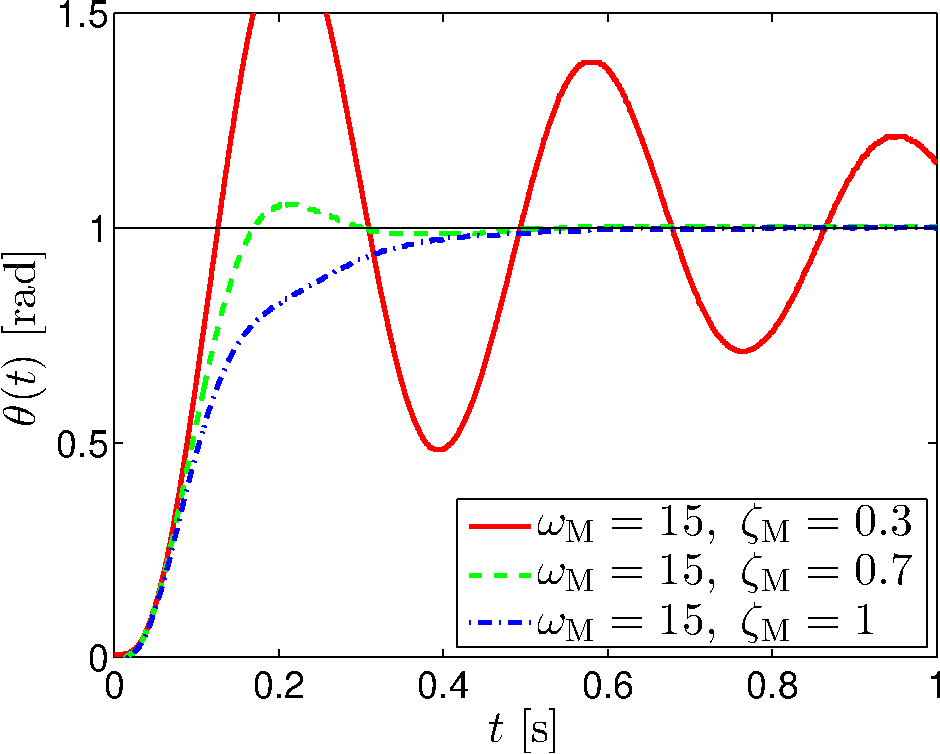
\includegraphics[scale=0.5]{sozai/figure_ipcont_angle-crop.pdf}
  \caption{ex\_ipcont}
\end{figure}

\begin{figure}[h]
  \centering
  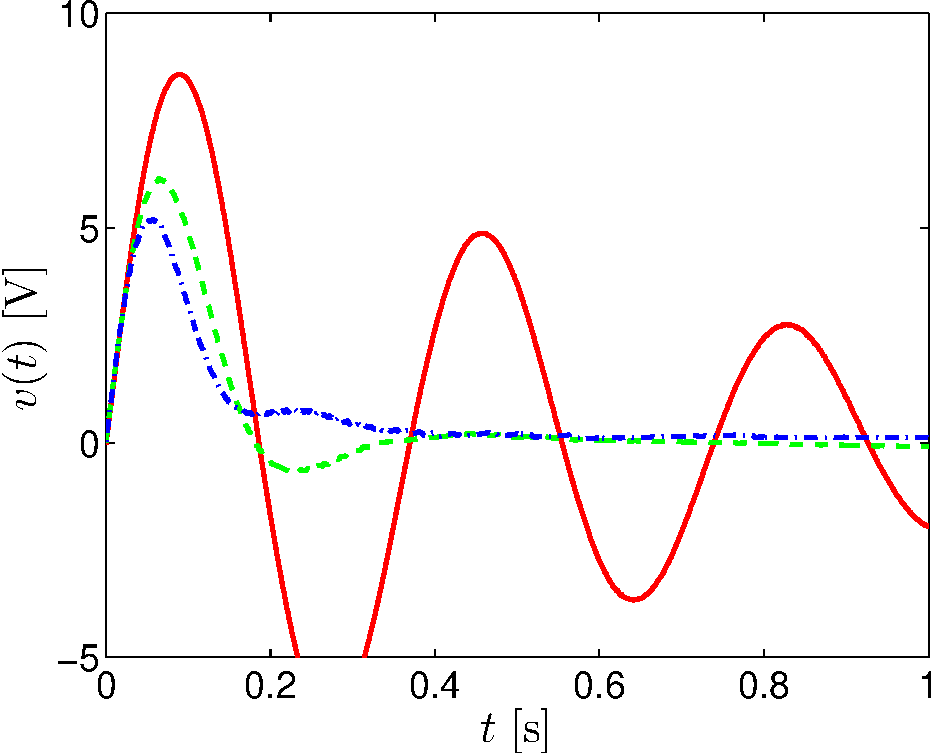
\includegraphics[scale=0.5]{sozai/figure_ipcont_volt-crop.pdf}
  \caption{ex\_ipcont}
\end{figure}

\newpage

\subsubsection{実験考察}
I-P制御は,偏差に積分動作を適用した量に基づいて,目標値の変化を滑らかにし,
その後に比例要素を作用させた操作量を出力します.
この制御構造により,I-P制御は目標値の急激な変化を緩和し,システムに与える影響を抑制する働きを持つ.
これは図5.9からも読み取れる.
P-D制御では積分動作がないため,外乱や負荷変動によって生じた定常偏差がそのまま残ってしまう一方,I-P制御
には積分動作が含まれているため,定常偏差が時間とともに収束し,最終的には目標値に到達する.
また,動作が規範モデルとことなる理由は,パラメータ調整に部分的モデルマッチング法が用いられているためである.
部分的モデルマッチング法は,特定の周波数帯域において理想モデルに近似するように設計されるが,
全体の応答を完全に再現するものではない.
したがって,高周波数成分や外乱の影響が含まれる実験結果においては,理想モデルと異なる結果が出たと考えられる.
また,PI制御には零点が含まれており,これによって特性が異なる.
具体的には,PI制御では零点の影響で応答が過渡的に速くなる傾向があるが,
I-P制御にはこの零点が存在しないため,応答はより滑らかで,
急激な変化が抑えられる.
この点で,I-P制御は目標値の変化に対して応答を穏やかにし,
システムが安定して追従するようになっている.


\subsection{I-PD制御}

\begin{enumerate}
  \item (4.22) 式にしたがって I-PD コントローラ (4.23) 式のパラメータを定め,表 5.4 を完成せよ.
        
  \item 次に,表 5.4 の比例ゲイン $k_{\mathrm{P}}$,積分ゲイン $k_{\mathrm{I}}$,微分ゲイン $k_{\mathrm{D}}$ を,コマンドウィンドウで次のように入力します.
        \begin{verbatim}
        kP = ***; kI = ***; kD = ***;
        \end{verbatim}
        
  \item Scope と Scope1 を開き,リアルタイムで角度と操作量を観測できるようにする.レジメは付録 A.2 の 図 A.8 に合わせる.
        
  \item センサ電圧が 0 [V] となる位置にアームを動かし,“ex\_ipdcont.slx” を実行する.実行終了後,コマンドウィンドウで
        \begin{verbatim}
  >> save ipdcont_data1 t u y kP kI kD
  \end{verbatim}
        と入力し,データを以下のファイルとして保存します.
        
        - “ipdcont\_data1.mat” ($\omega_M = 20, \alpha_{M1} = 2, \alpha_{M2} = 2$)
        - “ipdcont\_data2.mat” ($\omega_M = 20, \alpha_{M1} = 3, \alpha_{M2} = 3$)
        - “ipdcont\_data3.mat” ($\omega_M = 20, \alpha_{M1} = 2.15, \alpha_{M2} = 1.75$)
        
        これらの mat ファイルをディレクトリ D:\\\$student\_55\\group01\\ipdcont に保存します.最後に,以下の M ファイルを実行します.
        
        - “autoplot\_ipdcont.m”
        
        この実行によって,MATLAB 上でグラフを作成し,グラフの pdf ファイルは自動的に生成されます.
\end{enumerate}

\subsubsection{実験結果}
\begin{figure}[h]
  \centering
  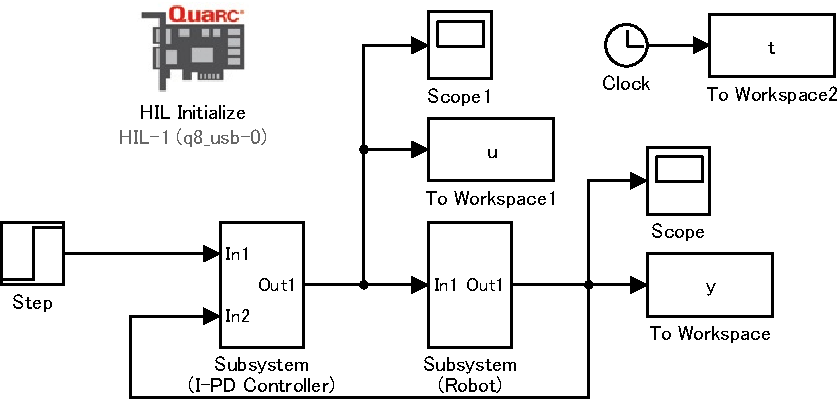
\includegraphics[scale=1]{sozai/ex_ipdcont-crop.pdf}
  \caption{ex\_ipdcont}
\end{figure}

\begin{table}[H]
  \centering
  \caption{I-PD コントローラ}
  \begin{tabular}{|c|c|c|c|c|c|}
    \hline
    $\omega_M$ & $\alpha_{M1}$ & $\alpha_{M2}$ & 比例ゲイン $k_{\mathrm{P}}$ & 積分ゲイン $k_{\mathrm{I}}$ & 微分ゲイン $k_{\mathrm{D}}$ \\ \hline
    20         & 2             & 2             & 25.157                      & 251.572                     & 0.575                       \\ \hline
    20         & 3             & 3             & 37.736                      & 251.572                     & 1.204                       \\ \hline
    20         & 2.15          & 1.75          & 27.044                      & 251.572                     & 0.418                       \\ \hline
  \end{tabular}
\end{table}


\begin{figure}[h]
  \centering
  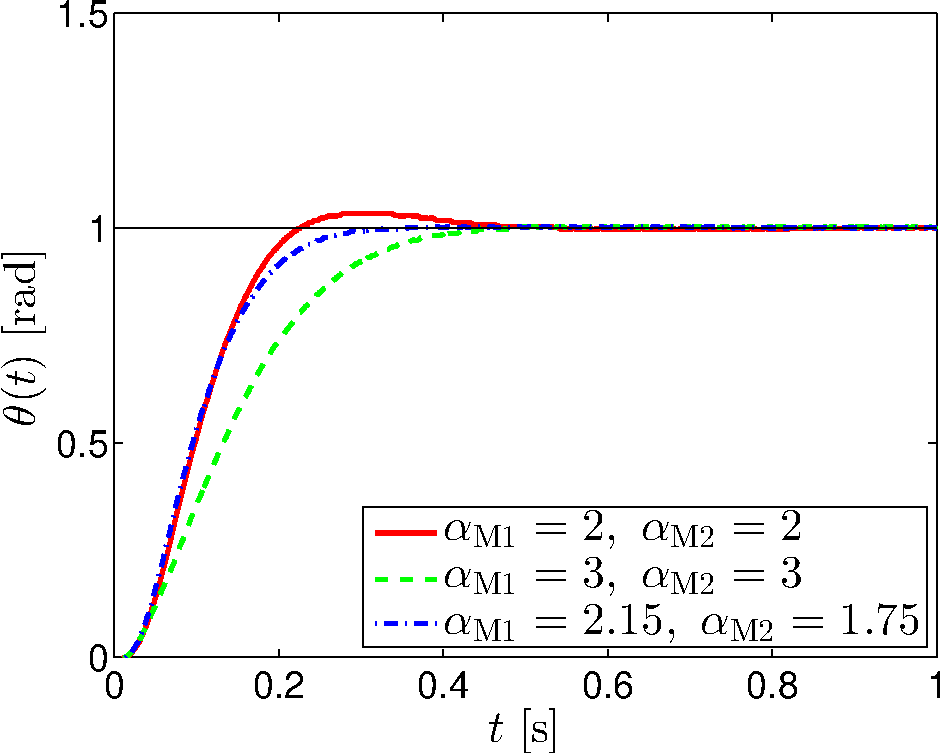
\includegraphics[scale=0.5]{sozai/figure_ipdcont_angle-crop.pdf}
  \caption{figure\_ipdcont\_angle}
\end{figure}

\begin{figure}[h]
  \centering
  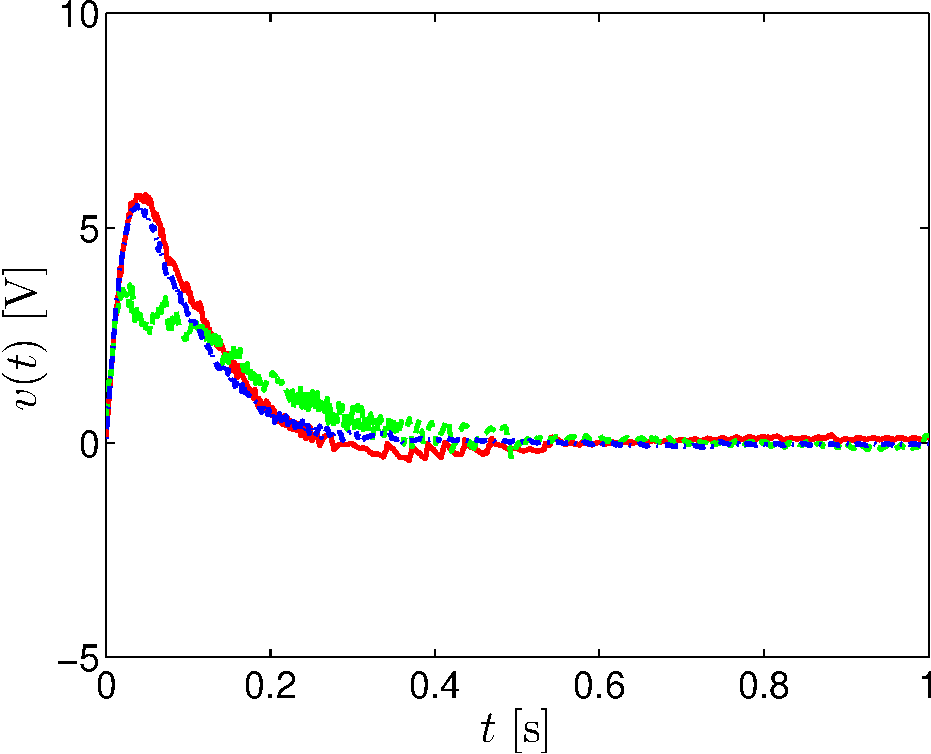
\includegraphics[scale=0.5]{sozai/figure_ipdcont_volt-crop.pdf}
  \caption{figure\_ipdcont\_volt}
\end{figure}

\newpage

\subsubsection{実験考察}
I-PD制御は,比例項(\( k_{\mathrm{P}} \))と積分項(\( k_{\mathrm{I}} \)),
および微分項(\( k_{\mathrm{D}} \))が組み合わさることで,
応答速度と定常精度が良くなっている.
図5.12より,角度応答では目標値への到達が速く,
また定常状態での偏差がほとんどないことがわかる.
これは積分項によって定常偏差が補正されるため,P-D制御と比較して定常偏差がほぼなくなっているためだと考えられる.
また,I-P制御と比較しても過渡応答が速く,振動が抑えられている.

一方で,図5.13に示される電圧応答においては,微分ゲインが大きいときに振動が見られる.
これは微分項が高周波成分やノイズに敏感であるためであり,
急激な変動に対して過大な操作量が発生しやすいためである.
そのため,一般的に微分動作の前にローパスフィルターなどのフィルターを通すことが一般的である.


\section{調査課題}

\subsection*{1}
ポテンショメータは,可変抵抗器の一種であり,
主に位置や角度を測定するためのセンサとして使用される.
その動作原理は,接点(スライダー)を抵抗体上で移動させることによって,
抵抗値を変化させ,その変化によって位置や角度を検出する.
抵抗体の両端に電圧を印加し,スライダーの位置に応じた電圧が出力されるため,位置情報が得られる.
\[
  \text{出力電圧} = \frac{\text{スライダーの位置}}{\text{全抵抗体の長さ}} \times \text{印加電圧}
\]
また,ポテンショメータはアブソリュート位置センサであるため,
電源のオン・オフに関係なく位置情報を保持できる.
しかし,スライダーと抵抗体の接触部分が摩耗しやすいため,
耐久性や寿命が求められる用途には不向きである.

\subsection*{2}
A/D変換は,アナログ信号をデジタル信号に変換するプロセスである.
アナログ信号が時間的および値の上で連続的であるのに対し,
デジタル信号は離散的なサンプル点と有限のビットで表現される.
まず,サンプリングにより,アナログ信号の時間的に連続したデータを一定の時間間隔で分割して離散化する.
次に,量子化を行う.
量子化は,サンプリングによって得られた信号の値を有限のビット数で表現できるように離散化するプロセスである.
量子化の精度はビット数に依存し,ビット数が多いほどより詳細なアナログ信号の情報を保持できる.
最後に,符号化が行われ,量子化された値をデジタル形式として記録する.
D/A変換は,デジタル信号を再びアナログ信号に戻すプロセスである.
デジタル信号は不連続なデータで構成されているため,
変換によって生成されるアナログ信号は理想的な連続信号とは異なる場合があるが,
近似的な再現が可能である.


\subsection*{3}
レンジが \(\pm 5\) V,分解能が12ビットの場合,アナログ出力の電圧は,
\[
  \text{1 LSB} = \frac{10 \, \text{V}}{4096} = \frac{10}{4096} \approx 0.00244 \, \text{V}
\]
次に,0x0C00のデジタル値をアナログ値に変換する.0x0C00は10進数に直すと3072であるため,

\[
  \text{アナログ値} = (3072) \times 0.00244 \, \text{V} - 5 \, \text{V} = 2.5 \, \text{V}
\]

よって0x0C00をD/A変換するとアナログ値は2.5[V]となる

\subsection*{4}
式 \(4.9\) は以下の通りである.
\[
  T(s) = \frac{\omega_n^2}{s^2 + 2 \zeta \omega_n s + \omega_n^2}, \quad \omega_n = \sqrt{b k_{\mathrm{P}}}, \quad \zeta = \frac{a + b k_{\mathrm{D}}}{2 \omega_n}
\]
システムの運動方程式に比例微分(PD)制御を適用すると,次の式が得られる.
\[
  m \frac{d^2 x}{dt^2} + c \frac{dx}{dt} + kx = k_{\mathrm{P}} e + k_{\mathrm{D}} \frac{de}{dt}
\]
ここで,簡略化のために \( b = \frac{1}{m} \) および \( a = \frac{c}{m} \) とおくと,上記の式は次のように表される.
\[
  \frac{d^2 x}{dt^2} + a \frac{dx}{dt} + bx = b k_{\mathrm{P}} e + b k_{\mathrm{D}} \frac{de}{dt}
\]

ラプラス変換を適用して,ラプラス変数 \( s \) を用いて表現する.これにより次の式が得られる.
\[
  (s^2 + as + b) X(s) = b k_{\mathrm{P}} E(s) + b k_{\mathrm{D}} s E(s)
\]
ここで,出力と入力の比 \( T(s) = \frac{X(s)}{E(s)} \) を整理すると,以下の伝達関数が得られる.
\[
  T(s) = \frac{X(s)}{E(s)} = \frac{b k_{\mathrm{P}} + b k_{\mathrm{D}} s}{s^2 + as + b}
\]

ここで,自然周波数 \( \omega_n \) と減衰係数 \( \zeta \) を次のように定義する.
\[
  \omega_n = \sqrt{b k_{\mathrm{P}}}
\]
\[
  \zeta = \frac{a + b k_{\mathrm{D}}}{2 \omega_n}
\]

これらを代入し,伝達関数を整理すると次の式が得られる.
\[
  T(s) = \frac{\omega_n^2}{s^2 + 2 \zeta \omega_n s + \omega_n^2}
\]


式 \(4.20\) は次のように与えられる.
\[
  T(s) = \frac{b k_{\mathrm{I}}}{s^3 + (a + b k_{\mathrm{D}})s^2 + b k_{\mathrm{P}} s + b k_{\mathrm{I}}}
\]
PID制御を適用したシステムの運動方程式は,次のように与えられる.
\[
  m \frac{d^2 x}{dt^2} + c \frac{dx}{dt} + kx = k_{\mathrm{P}} e + k_{\mathrm{D}} \frac{de}{dt} + k_{\mathrm{I}} \int e \, dt
\]
ここで,簡略化のために \( b = \frac{1}{m} \) および \( a = \frac{c}{m} \) とおくと,上記の式は次のように書き直される.
\[
  \frac{d^2 x}{dt^2} + a \frac{dx}{dt} + bx = b k_{\mathrm{P}} e + b k_{\mathrm{D}} \frac{de}{dt} + b k_{\mathrm{I}} \int e \, dt
\]

ラプラス変換を適用して,ラプラス変数 \( s \) を用いて表現すると,積分項 \( \int e \, dt \) のラプラス変換は \( \frac{E(s)}{s} \) となり,以下の式が得られる.
\[
  (s^2 + as + b) X(s) = b k_{\mathrm{P}} E(s) + b k_{\mathrm{D}} s E(s) + \frac{b k_{\mathrm{I}}}{s} E(s)
\]

次に,この式を \( X(s) \) と \( E(s) \) の関係として整理する.右辺を \( E(s) \) でくくり出すと,以下のようになる.
\[
  (s^2 + as + b) X(s) = \left( b k_{\mathrm{P}} + b k_{\mathrm{D}} s + \frac{b k_{\mathrm{I}}}{s} \right) E(s)
\]

ここで,\( T(s) = \frac{X(s)}{E(s)} \) として,両辺を \( E(s) \) で割ると次のようになる.
\[
  T(s) = \frac{X(s)}{E(s)} = \frac{b k_{\mathrm{I}}}{s^3 + (a + b k_{\mathrm{D}}) s^2 + b k_{\mathrm{P}} s + b k_{\mathrm{I}}}
\]